%# -*- coding: utf-8-unix -*-
%%==================================================
%% chapter_4.tex for SJTU Master Thesis
%%==================================================

\chapter{基于神经网络及PID控制的时钟伺服系统可行性研究}
在第\ref{chap:statistical_delay}章中,本人从链路传输延时的角度,通过深入分析实际工业环境下对链路传输延时的影响,通过对链路传输延时建立细致的数学模型,并从数学统计的角度对其中各个影响因素提出了有针对性的解决方案。

至此,我们已经能够利用上述算法综合获得稳定和精确的链路延时。但是,仅仅获取稳定精确的链路延时并不是时钟同步的终点。而且,在现实IEEE1588协议运行中,之所以同步精度难以达到亚微秒的同步精度,有很重要的因素是从时钟校正策略的选取。所谓时钟同步,最核心一环自然是从时钟根据计算数据对本地进行校正来实现同步,即时钟伺服系统。

常规我们在IEEE1588协议中采用的是PI控制策略,即利用PI控制器来对从时钟进行校正,而不是直接利用offset进行校正。这种做法能够一定程度提高从时钟的同步精度和稳定性,但它也存在如PI参数固定等缺陷而导致同步系统无法有效应对复杂多变的工业网络环境,这严重破坏了从时钟系统的鲁棒性和稳定性。因此,考虑到工业网络环境的复杂性和多变性,本文尝试从神经网络控制策略入手,以期待利用神经网络优秀的适应性来提高从时钟对复杂环境的鲁棒性和自适应性。

\section{时钟伺服系统研究}
对从时钟而言,如果想要实现与主时钟同步,就必须依靠前面提到的同步算法及所计算出来的链路时延值,从而对从时钟自身的相位和频率进行校正,以有效消除与主时钟之间的偏差。不过,由于当前的很多工业平台并非实时操作系统,所以一般而言都需要利用中断机制来触发从时钟进行校正。但是,在该中断过程中造成的从时钟漂移抖动会长期破坏同步精度,严重影响同步过程的实时性。

因此,为了提高从时钟校正过程的实时性和快速性,我们需要设计一套比较良好的时钟伺服系统来对从时钟进行校正。

\subsection{通用PTP时钟伺服系统介绍}

\begin{figure}[!hbp]
  \centering
  \begin{minipage}[b]{0.7\textwidth}
    \captionstyle{\centering}
    \centering
    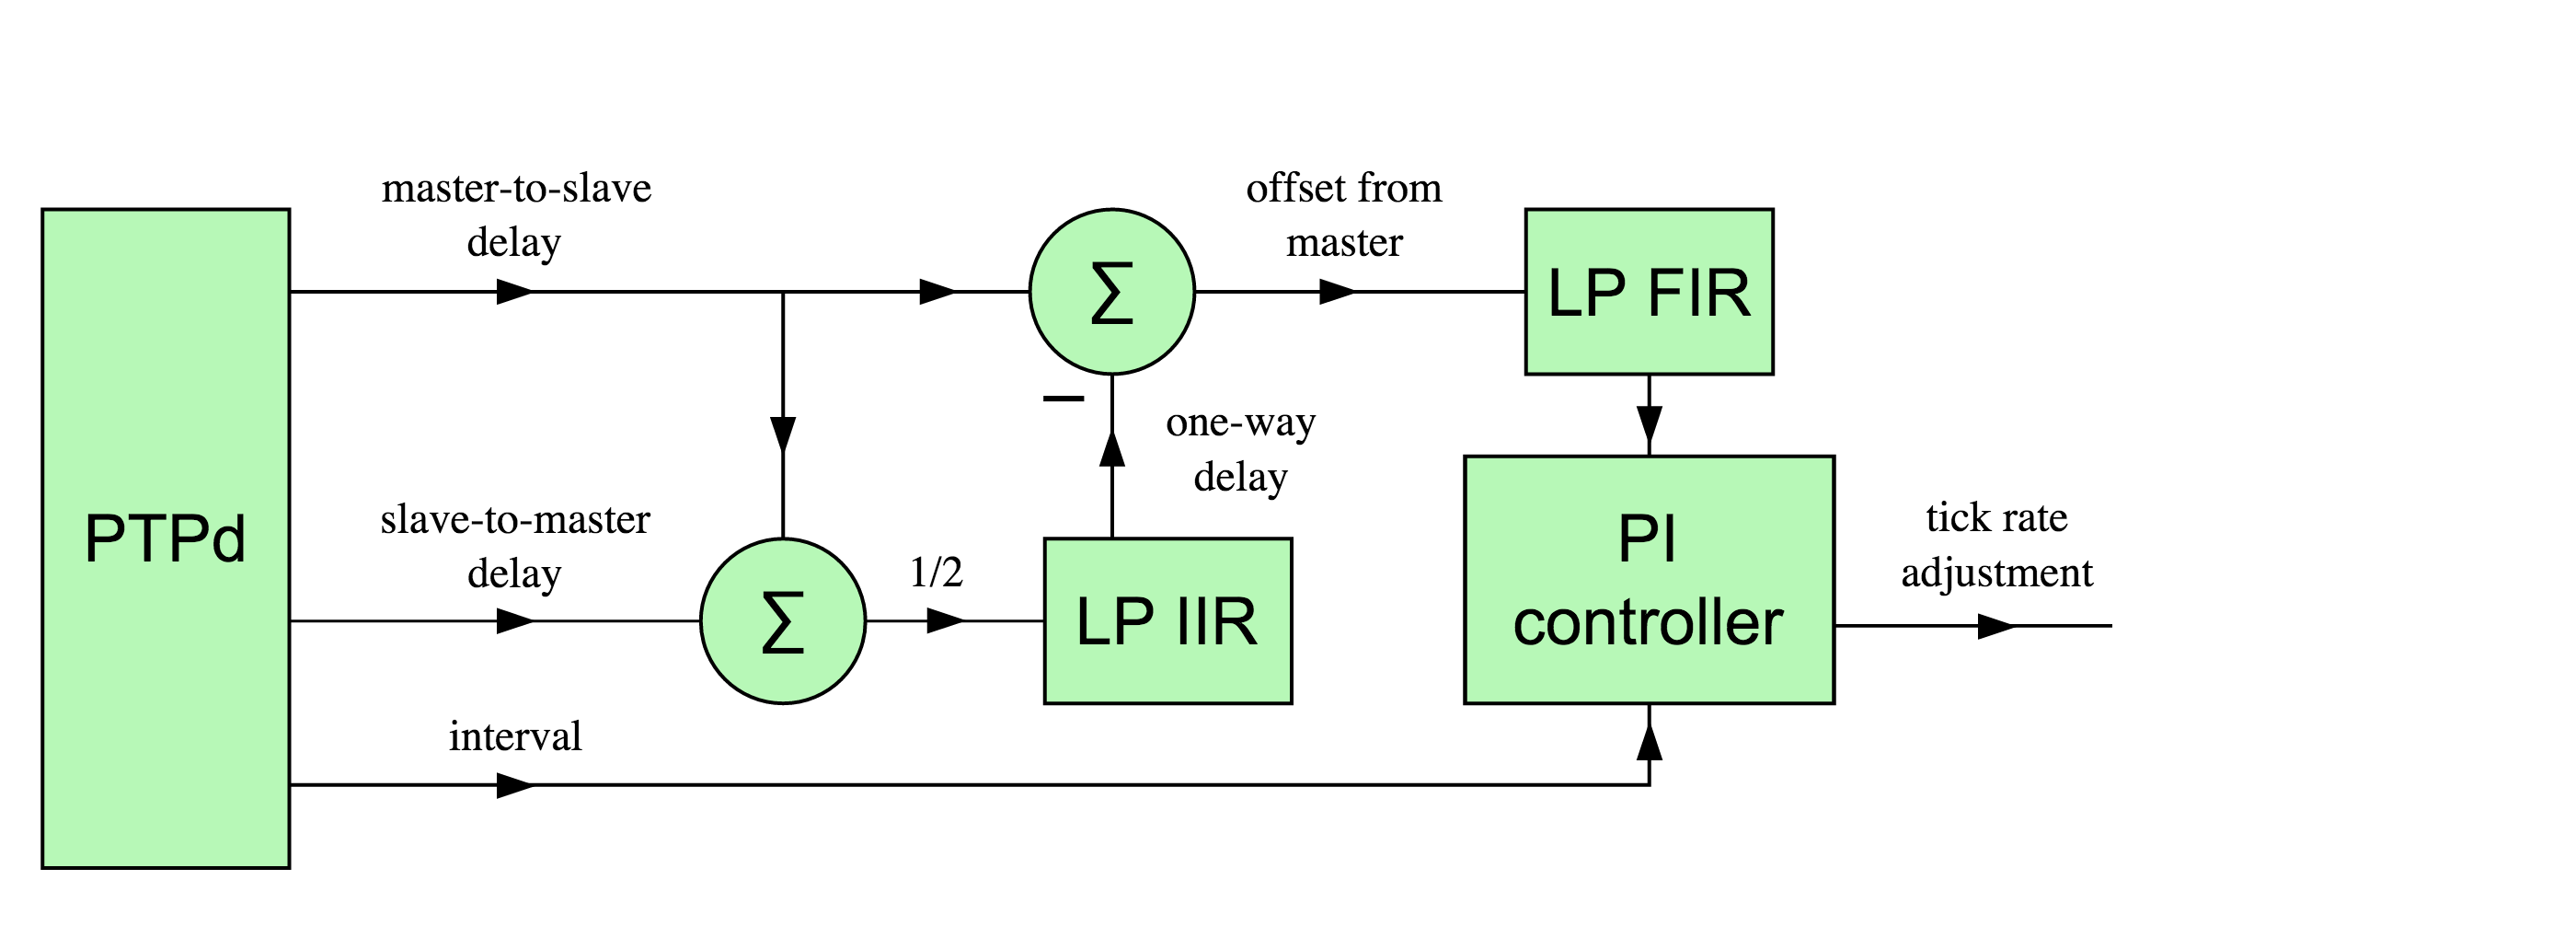
\includegraphics[width=11cm]{normal_clock_servo_system}
    \bicaption[fig:normal_clock_servo_system]{通用PTP时钟伺服系统}{通用PTP时钟伺服系统}{Fig}{The normal structure of general PTP clock servo system}
  \end{minipage}     
\end{figure}

一种常见的PTP时钟伺服系统如上图\ref{fig:normal_clock_servo_system}所示。从左到右表明了数据从PTP协议引擎逐渐流向从时钟。在该系统中,PTP协议引擎通过周期性获取主从偏差和从主偏差,将这两个偏差值通过均值滤波及低通滤波器获取到当前offset值。然后,将当前offset值与采样周期数据共同传递给PI控制器,由PI控制器来对从时钟进行校正以实现主从同步。该PI控制器由比例(P)和积分(I)两个环节共同构成,其中,比例环节可以用来消除主从时钟间的相位偏差,而积分项则可以用来消除系统的稳态误差,即消除主从时钟间的频率差。

上述这样一套较为完整的时钟伺服系统可以较好的实现时钟同步,而且,由于传统的PI控制算法相对而言比较简单、鲁棒性良好且可靠性较高,所以传统的PI控制器在工业控制领域里应用十分广泛。

但是,传统的PI控制器也有其固有的弊病,那就是其比例积分参数的调整往往需要依靠经验来设定。对于处于复杂网络环境中的时钟同步系统而言,仅仅依靠经验来整定控制参数的PI控制器几乎无法应对任何形式的复杂多变的环境,尤其是同步系统中的网络环境中存在多种非线性、时变性等不确定性因素时,被控对象特性常常会随着时间发生变化。例如工业中充当从时钟的PTP设备,很容易会随着时间慢慢精度降低,并且长期受到工业干扰导致设备性能逐渐下降。这些从时钟的变化都会导致传统的PI控制器在时钟伺服系统中无法达到良好的控制效果。

所以,为了使得时钟伺服系统能够适应工业网络环境变化,尤其是应对时变性非常强的网络传输环境,本人在下文从智能自适应控制的角度出发,结合同步系统特性进行深入分析,并且提出基于智能控制策略作为伺服系统中的控制环节,从而来弥补传统PI控制器无法适应复杂网络环境的缺陷。

\subsection{智能控制策略介绍}
随着被控对象及控制环境的越来越复杂,很多智能控制策略也相继出现,并且已经广泛应用到了工业网络控制系统中。以网络控制系统中的时延不确定性为例,当前工业中陆续采用了多种智能控制方法来提高系统的鲁棒性和抗干扰性\supercite{19,20}。文献\parencite{21}中,作者通过对实际的Internet控制系统的时延数据分析,从而对控制系统建立了状态反馈模糊控制器;文献\parencite{22}采用了动态模糊控制器,对基于TCP/IP网络的远程伺服控制系统进行了研究;文献\parencite{23}中作者针对Ethernet提出了一种改进型神经元PID控制器,该控制器可以不依赖于网络时延精确数学模型。这些研究成果都表明对于复杂的网络环境,我们可以采用智能控制策略来进行自适应控制,而且能够取得良好的控制效果。

\section{基于神经网络的PID控制策略}
根据上节可以知道,由于传统PI控制器无法适应网络传输环境和被控对象的时变性,我们需要采用一种能够自动根据当前网络环境而调整的控制策略。本人在此选择神经网络及PI控制相结合,以此来实现时钟伺服系统中对从时钟的控制。下文会对该控制策略进行详细讲解。

\subsection{神经网络介绍与研究}
\subsubsection{神经网络特征}
神经网络\footnote{Neural Network}是由大量处理单元(神经元)广泛互联而成的网络,它基于人类对大脑工作机理的认识,以人脑的组织结构和活动规律作为背景,而且能够反映人脑的一定基本特征。我可以认为,神经网络就是对人脑的某种抽象、简化和模仿。简单而言,神经网络是一个数学模型,可以用计算机来模拟甚至用电子器件来模拟人的智能,主要更根植于神经科学、统计学、数学、计算机科学等多种学科。另外,神经网络不仅是高度非线性动力学系统,又是自适应系统,可以用来描述认知决策和控制等智能行为。

神经网络具有存储和应用经验知识的主要特征,与人脑相比,它具备以下两个相似之处:
\begin{itemize}[noitemsep,topsep=0pt,parsep=0pt,partopsep=0pt]
	\item 可以通过学习来从外部环境中获取知识,即使在不断变化的复杂环境下,它仍然能够通过不断的学习来适应这种环境的变化。
	\item 内部神经元具有存储知识的能力,只要神经网络对某种环境进行了学习,那么所积累下来的经验就会一直存在于神经网络内部,并且会在未来的继续学习中不断调整和改良。
\end{itemize}

\subsubsection{神经网络基本原理及构造}
神经网络作为模拟人的思维方式,用以实现多位数据的表示,其内部单元大都使用结构简单的神经元模型,通过内部神经元之间的相互关联及权值修正来实现对多维数据的非线性处理。

\begin{figure}[!hbp]
  \centering
  \begin{minipage}[b]{0.6\textwidth}
    \captionstyle{\centering}
    \centering
    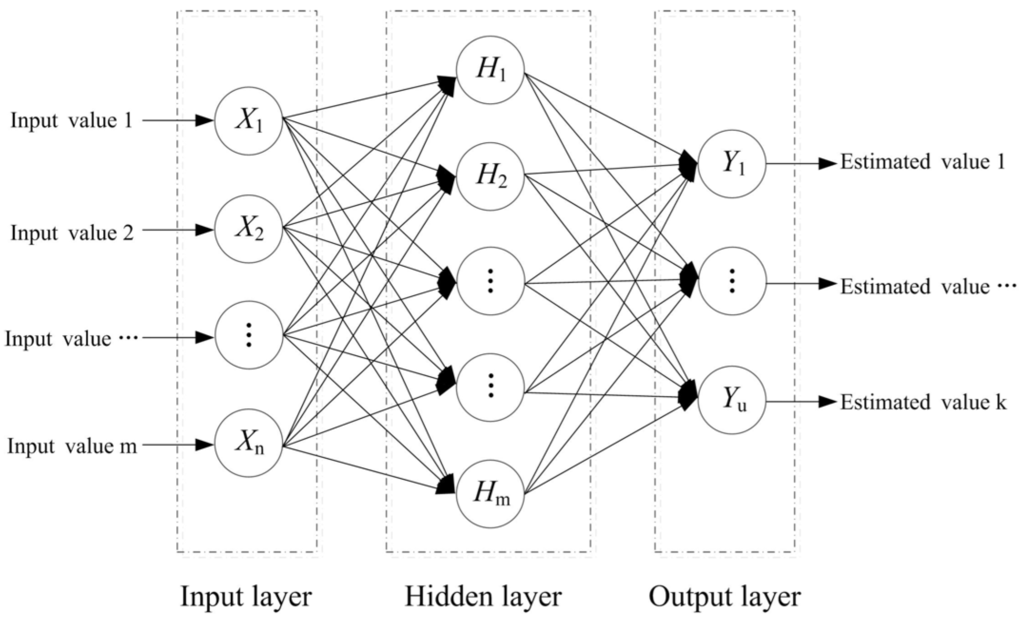
\includegraphics[width=10cm]{neural_network}
    \bicaption[fig:neural_network]{神经网络结构图}{神经网络结构图}{Fig}{The structure of neural network}
  \end{minipage}     
\end{figure}

根据图\ref{fig:neural_network}可以看到神经网络的整体结构,在一套完整的神经网络结构中,一般会包含多个不同的网络层单元,即下列几个网络层:
\begin{itemize}[noitemsep,topsep=0pt,parsep=0pt,partopsep=0pt]
	\item 输入层(Input Layer):这一层的输入节点主要对应外部数据的特征变量,为了能够有效地描述外界事物,我们需要对研究对象选择特定且有意义的原始特征变量,或者称为特征空间。所以说,这一层中会有大量神经元接受外界复杂的非线性输入信息。
	\item 隐含层(Hidden Layer):这一层是中间层,简称“隐层”,是输入层和输出层之间众多神经元和链接组成的各个层面。隐层可以有多层,习惯上会用一层。隐层的节点(神经元)数目不定,但数目越多神经网络的非线性越显著,从而神经网络的强健性(robustness)(控制系统在一定结构、大小等的参数摄动下,维持某些性能的特性。)更显著。习惯上会选输入节点1.2至1.5倍的节点。
	\item 输出层(Output Layer):这一层是神经网络经过计算后将计算值对外输出的一层。所有原始数据在神经元链接中传输、分析、权衡,形成输出结果。所输出的信息称为输出向量。
\end{itemize}

\subsubsection{神经网络训练过程}
以“聚类”为例子,为了将具备相同属性的对象归为同一类,首先,神经网络方法会将每个簇描述为一个标本,此处的标本不一定对应一个特定的数据实例或者对象。然后,神经网络会根据某些距离度量,把新的对象分配给标本与其最相似的簇,在一个簇内部,所有对象的属性可以根据该簇标本的属性来预测。在神经网络内部的处理单元,会采用一系列的数学函数,通过将这些函数进行汇总和转换,来对数据进行处理。而且,此处可以将多个处理单元连接称为系统,即可以创建一个智能模型。

在神经网络开始训练之前,需要将处理单元和输入/输出单元连接起来。训练过程中,会对输入元和输出元之间的连接强度,或者说权值,进行修改。具体的修改方式要依据其对某一结果的重要程度来进行调解。在这里,我们会采用一种称为学习规则的数学方法来调节权值。

神经网络的训练是根据历史样本数据反复进行的,训练时会对处理单元之间连接的权值不断修改。或者说,为了对每一个样本的结果变量进行预测,它会尝试各种不同的方案。当输出的结果在指定的精度级别上与已知结果相吻合时,那么就停止网络的训练。

\subsection{神经网络与时钟伺服系统的关联性研究}
之所以本文会采取神经网络作为时钟伺服的控制学习策略,主要基于以下几点考虑:
\begin{itemize}[noitemsep,topsep=0pt,parsep=0pt,partopsep=0pt]
	\item 神经网络是高度非线性动力学系统,又是自适应自组织系统,而我们的时钟同步系统所在的工业网络环境也是非常复杂且时变的,所以,我们需要一个学习策略能够根据外界网络环境的变化来调节自身,具备良好自适应性。因此,神经网络是一个很好的选择。
	\item 神经网络具备学习功能,即通过学习大量的样本数据来获取输入输出之间的函数关系,这对于数学模型复杂或难以建立的系统具备良好的适应性,而我们的从时钟系统便由于工业现场的多变性而难以建立准确的数学模型。因此,神经网络能够发挥样本数据的优势来解决。
	\item 神经网络作为数据非线性映射工具,和基于传统统计的数学方法并不矛盾,而且二者可以互相补充。由上文介绍知道,本文中采用了多种数学统计方法,也积累了很多样本数据,因此,数学统计策略与神经网络模型可以良好的结合在一起。
\end{itemize}

因此,由于神经网络高度的自学习能力,非常适合模拟复杂的非线性系统。根据神经网络理论中的Kolmogorov连续性定理,给定任一连续函数
\begin{align}
f:[0,1] \quad n \rightarrow Rm
\end{align}
f可以精确地用一个三层前馈神经网络来实现,从数学上保证了神经网络用语时间序列预测的可行性。而且,本文中采用了多种数学统计方法,积累了很多的样本数据,而神经网络作为数据非线性映射工具,可以和前面所提的数学统计方法得到非常良好的结合。

\subsection{BP神经网络原理}
1985年,Rumelhart等人提出的BP反向传播算法\footnote{back propagation}是一种多层前馈网络所使用的有监督的学习过程。该算法主要依据给定的(输入、输出)样本来进行学习,并且通过计算网络的实际输出值与期望输出的误差反馈偏差,利用该偏差值来对网络连接权值进行调整,最终达到学习的目的。误差反向传播学习算法通常是按照最小均方差的准则,使用梯度下降法在误差曲面搜索误差函数的极小值,然后通过调整连接权值来使该误差函数极小化。具体有如下几个步骤:
\begin{enumerate}[noitemsep,topsep=0pt,parsep=0pt,partopsep=0pt]
	\item 输入样本,并使用事先确定的激励函数计算各结点的实际输出值:
	 	\begin{align}
	 		O = f(\omega \cdot x)
	 	\end{align}
	 	Sigmoid函数是一类激励函数在应用中最普遍的函数,[0,1]上的Sigmoid函数表达式及导数为:\\
	 	原函数形式:
	 	\begin{align}
	 		f_{1}(x) = \frac{1}{(1 - exp(-\lambda x))}
	 	\end{align}
	 	导数形式:
		\begin{align}
	 		f_{1}'(x) = \lambda f_{1}(x)[1-f_{1}(x)]
	 	\end{align}
	 \item 使用以下的误差函数公式计算神经网络输出与期望之间的均方差:
	 	\begin{align}
	 		E(\omega) = 0.5\sum_{k\in Input Layer}(t_{k} - o_{k})^{2}
	 	\end{align}
	 	在上式中,样本的期望输出值表示为$t_{k}$,对于网络输出层的第k个结点的实际输出值为$o_{k}$,其中k为网络层输出节点。
	 \item 通过反向传播的计算方法,计算输出层中每个输出节点的误差项:
	 	\begin{align}
	 		\delta_{k} = o_{k}'(t_{k} - o_{k}) = o_{k}(1 - o_{k})(t_{k} - o_{k})
	 	\end{align}
	 \item 对于隐含层中的每个隐含节点,计算当前输出情况下其对应的误差项:
	 	\begin{align}
	 		\delta_{h} = o_{h}'\sum_{k}\omega_{hk}\delta_{k} = o_{h}(1 - o_{h})\sum_{k}\omega_{hk}\delta_{k}
	 	\end{align}
	 	其中,k表示输出的节点,h表示内部隐含层的神经元节点。
	\item 计算各连接权的修正值,其中$\eta$ 是学习率,较小的$\eta$ 可以保证训练能更稳定的收敛,但会消耗比较长的收敛时间;
	反之,较大的$\eta$可以在提高一定的收敛速度,但是,这可能会导致系统不稳定。
	 	\begin{align}
	 		\Delta \omega_{ji} = \eta \delta_{j} x_{ji}
	 	\end{align}
	 \item 依据上一步的计算结果,可以对各连接权的权值进行调整,然后继续从第一步开始处理。
	 	\begin{align}
	 		\omega_{ji} = \omega_{ji} + \Delta\omega_{ji}
	 	\end{align}
	 	当响应单元的输出值接近0或1时,Sigmoid导数的值将接近于0、1。
\end{enumerate}

\subsection{BP神经网络的改进}
在对称型Sigmoid激励函数的神经网络中,当响应单元的输出值接近-1或1时也存在类似现象,这样的区域被称为饱和区域。由于Sigmoid导数值用于反馈误差中的修正值计算,当Sigmoid函数进入饱和区域时,在权值修正公式中的权值修正量就变的微乎其微了,这样就导致网络的训练陷入了饱和状态之中,这使得学习效率大大降低了。所以,为了修正BP神经网络中的这些固有缺陷,一般会从一下两种角度来进行改进:一种是基于标准数值最优化的改进方法,如共轭梯度算法、拟牛顿算法和LM算法\footnote{Levenberg-Marquardt};另一种是基于标准梯度下降的改进方法,如增加动量项的BP算法、自适应学习速率法和弹性BP算法等。下面主要对增加动量法作简单介绍。

标准的BP算法实质是一种简单的最速下降静态寻优算法,在修正权值$\omega(k)$时,只是按照当前时刻的负梯度方式进行修正,而没有考虑以前积累的经验,即以前时刻的梯度方向,从而有可能导致学习过程中收敛较为缓慢,甚至发生振荡。所以,为了改进这一点,我们可以将上一次权值调整值的一部分迭加到本次误差计算所得的权值调整量上,以作为本次的实际权值调整量,使BP神经网络在修正权值时,不仅考虑误差在梯度上的作用,而且考虑其对于误差曲面变化趋势的影响。即:
\begin{align}
	\omega(k+1) = \omega(k) + \eta[(1-a)D(k) + aD(k-1)]
\end{align}
其中,$\omega(k)$表示当前时刻的权值向量,D(k)表示负梯度方向k训练阶段的值为学习率,最重要的是在这个学习过程中引入了a系数,我们称之为动量因子,
\begin{align}
	a \in [0, 1]
\end{align}
当神经网络在附加动量因子的方法下进行训练时,a参数既能帮助减小学习过程的振荡趋势,有能够降低网络对于误差曲面局部细节的敏感性,这有效地抑制网络陷入局部极小的状态,从而使的系统有更好的收敛性和更优的解。

\section{基于BP神经网络的PID控制策略实现}
由上文可知,对于时钟同步系统而言,由于工业网络环境复杂且时刻变化,简单的PI控制完全无法应对多变的环境,也不具备任何自适应性。所以,仅仅采用简单的PI控制无法使的从时钟系统能够达到很好的稳定性和收敛性,甚至可能由于网络环境的不断变化而发生振荡甚至难以稳定。因此,一种能够控制非线性且时变的对象的控制策略对于工业环境下时钟同步系统而言至关重要。

在上一小节中,本人通过对神经网络基础原理及相关理论进行了较为深入的研究。可以看出,神经网络算法不仅具备良好的学习功能,这能帮助从时钟在复杂的网络环境下不断对自身进行调整以达到良好的同步效果,而且,该算法作为数据非线性映射工具,还能与传统统计方法相互补充,而本人在前面已经采取了多种统计算法,所以,在从时钟端会累积很多样本数据,这些样本的存在正好使的神经网络算法发挥更大的作用。

为了将神经网络算法应用于时钟伺服系统中,我们可以将神经网络与PID控制系统相结合,通过外界输入样本对神经网络进行训练,然后让神经网络对外输出PID控制系统所需要的三种控制参数$K_{i}$、$K_{p}$、$K_{d}$。可以参考下图的结构设计:

\begin{figure}[!hbp]
  \centering
  \begin{minipage}[b]{0.6\textwidth}
    \captionstyle{\centering}
    \centering
    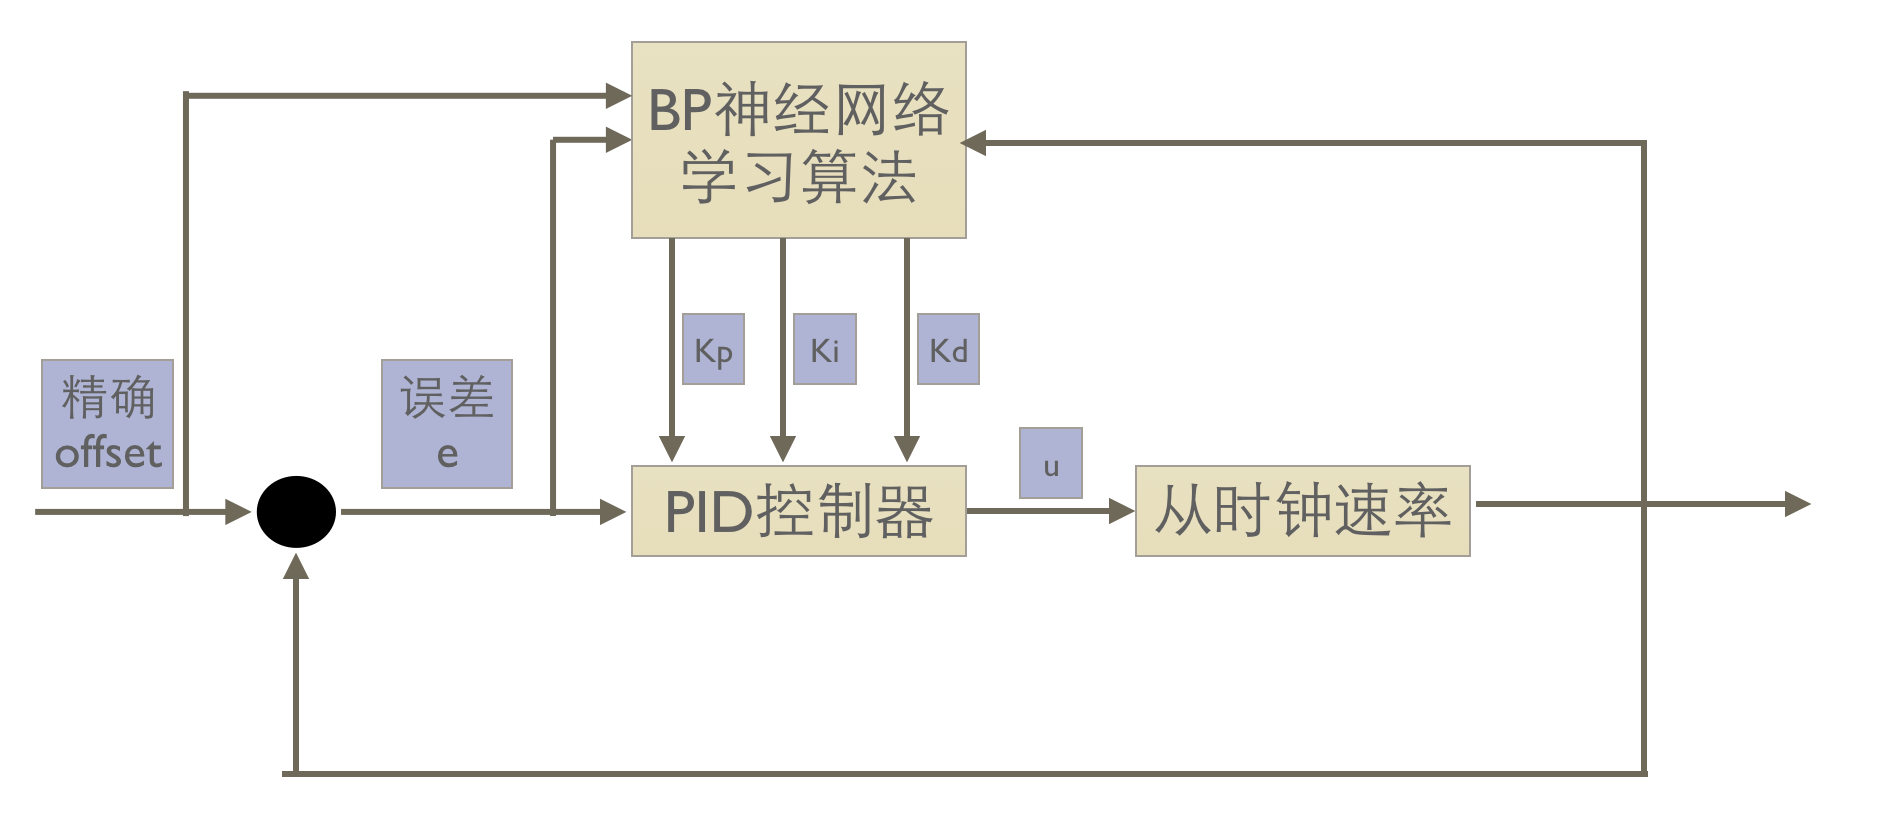
\includegraphics[width=10cm]{bp_neural_network_PID}
    \bicaption[fig:bp_neural_network_PID]{基于BP神经网络的PID控制系统结构图}{基于BP神经网络的PID控制系统结构图}{Fig}{The structure combining BP neural network with PID controller}
  \end{minipage}     
\end{figure}

\subsection{BP神经网络结构}
下图\ref{fig:bp_neural_network}为BP\footnote{Back Propagation 误差反向传播}神经网络结构图,从左往右依次为输入层、隐含层、输出层,下文将依据该结构,将伺服系统分成前向传播过程和误差反向传播过程来分别讲述。
\begin{figure}[!hbp]
  \centering
  \begin{minipage}[b]{0.6\textwidth}
    \captionstyle{\centering}
    \centering
    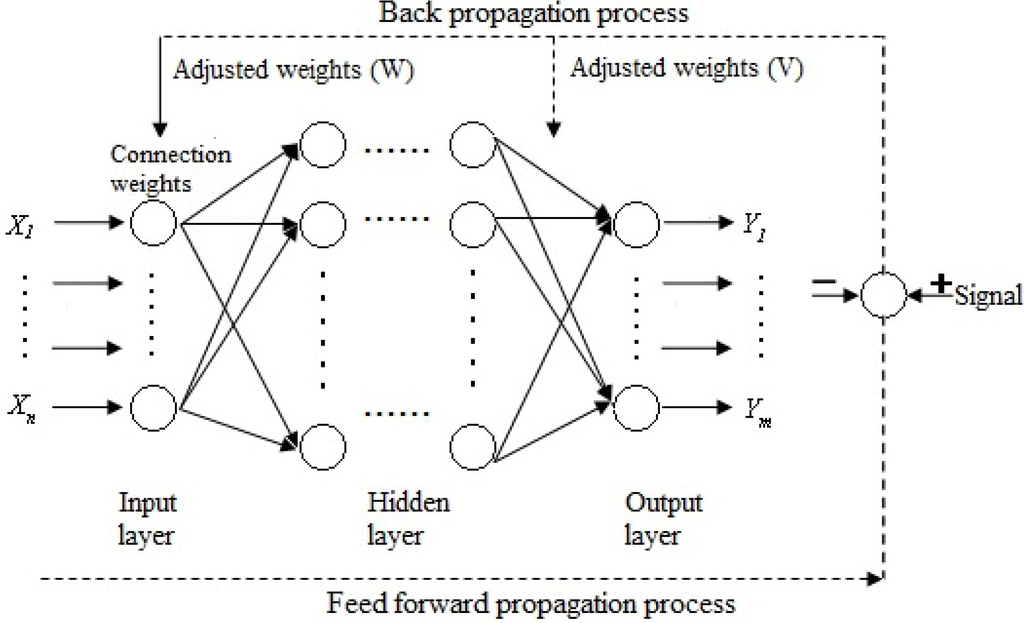
\includegraphics[width=10cm]{BP_neural_network}
    \bicaption[fig:bp_neural_network]{BP神经网络结构图}{BP神经网络结构图}{Fig}{The structure of BP neural network}
  \end{minipage}     
\end{figure}

\subsection{前向计算过程}
该过程是指输入变量依次经过输入层、隐含层直到输出层的过程。首先,对于输入层,我们可以选取k个主从偏差样本作为神经网络的输入。该样本个数k若太大,则会导致训练时间过长,系统需要较长时间的收敛过程;反之,若样本个数$K_{i}$太小,则会导致达不到学习效果。在此,本人将$K_{i}$选取为4。所以,输入层的输入为:
\begin{align}
	input_{1} = offset_{c}, input_{2} = offset_{(c-1)}, \\
	input_{3} = offset_{(c-2)}, input_{4} = offset_{(c-3)}, 
\end{align}
其中,$offset_{c}$是表示当前时刻计算得到的时延值。所以,在输入层第i个输入节点的输出值为:
\begin{align}
	InputLayer\_Output_{i} = input_{i} \qquad i = 1, 2, 3, 4
\end{align}

然后,在隐含层有$K_{h}$个神经元节点,那么假设对于隐含层的第j个神经元的输入为:
\begin{align}
	HiddenLayer\_Input_{j} = \sum_{j=1}^{K_{h}}(W_{ij}InputLayer\_Output_{i})
\end{align}
即每一个隐含层节点的输入为所有输入层节点输出值乘以权值的总和。我们可以得到其隐含层节点的输出值为:
\begin{align}
	HiddenLayer\_Output_{j} = f(HiddenLayer\_Input_{j}) \qquad j = 1, 2 \cdots K_{h}
\end{align}

最后,在输出层,我们只选取三个输出节点,这三个节点分别对外提供三个控制参数$K_{i}$、$K_{p}$、$K_{d}$。
\begin{align}
K_{o} = 3
\end{align}
对于其中第z个输出节点,可以得到其输入值为:
\begin{align}
OutputLayer\_Input_{z} = \sum_{j=1}^{K_{h}}(W_{jz}HiddenLayer\_Output_{j}) \qquad z = 1, 2, 3
\end{align}
同时,我们可以得到第z个输出节点的最终输出值为:
\begin{align}
OutputLayer\_Output_{z} = g(HiddenLayer\_Input_{j}) \qquad j = 1, 2 \cdots K_{o}
\end{align}
其中,我们依次取各个输出为如下对应控制参数:
\begin{align}
K_{p} = OutputLayer\_Output_{1}
K_{i} = OutputLayer\_Output_{2}
K_{d} = OutputLayer\_Output_{3}
\end{align}

在上面的几个方程中,我们用$W_{ij}$来表示输入层到隐含层加权系数,然后用$W_{jz}$来表示隐含层到输出层的加权系数。另外,对于活化函数有多种选择方式,本人对于输入层\-隐含层及隐含层\-输出层分别取下面两个活化函数:
\begin{align}
Log-Sigmoid : f(x) = \frac{1}{1 + e^{-x}} \\
Sigmoid : g(x) = \frac{e^{x} - e^{-x}}{e^{x} + e^{-x}}
\end{align}

至此,我们已经可以从输出层得到三个控制参数$K_{i}$、$K_{p}$、$K_{d}$。但是,目前得到的三个控制参数并不能保证系统稳定,我们还需要误差反向传播过程,将实际误差反向传回给神经网络,并依靠该误差来进行加权系数的校正。

\subsection{误差反向传播}
根据上文中,我们已经了解到了BP神经网络算法中的固有缺陷,同时本人已经在上文中介绍响应的改进算法,下面,我们就该增加动量法来进行反向传播调节的实际。

首先,我们依据最速下降法取性能指标函数为:
\begin{align}
T(k) = \frac{1}{2}(Rin(k) - Yout(k))^{2}
\end{align}
同时,我们利用近似最速下降法来更新该系统中的各个权值,具体的更新方法如下:
\begin{align}
\Delta W_{jz}(k) = -\eta \frac{\partial E(k)}{\partial W_{jz}} + \alpha \Delta W_{jz}(k-1)
\end{align}
在上式子中,$\alpha$用来表示惯性系数,$\eta$用来表示学习速度,式子的后半部分是指在k-1时刻网络权值的修改方向,这也正是上文中所介绍的增加动量法的权值更新方式。也就是说,如果第k次的更新方向与k-1次相同,那么后半部分就为正,从而加速整个更新过程,相反,如果二者方向不同,那么后半部分为负,从而起到稳定更新算法的作用。

\subsection{小结}
利用上述基于BP神经网络的PID控制器,通过神经网络与输入样本值来计算控制器所需的三个控制参数,从而实现对从时钟的校正。


% \section{IEEE1588协议在硬件上的实现}
% 在本文之前的部分中,本人已经从软件层面深入研究了链路延时及时钟伺服系统对整个时钟同步系统的影响,同时,分别针对链路传输延时抖动、“暂时性”时延突变、“持久性”时延变化和时钟伺服系统等多个角度分别提出了相应的优化方案,这些方案主要是从数学统计角度和智能控制的角度出发。这些方案的提出,不仅能够提高时钟同步精度,使其能够在复杂工业网络环境中达到亚微秒级,同时,也能够提高从时钟的稳定性和时钟同步的快速收敛性。

% 在本小结中,本人将结合自身在实验室所参与的实际工程项目,详细介绍如何将IEEE1588协议应用到实际硬件上,并且从硬件层面提出相应的提高时钟同步精度的措施。






